\scanpage{54}
\uline{Question} In 21) d) should one
strengthen the condition to
\[
(24)\quad\left\{\begin{aligned}
&\forall i,j\in I,\quad i\wedge j\overset{\mathrm{def}}{=}\operatorname{Inf}(i,j)\text{ exists, and}\\
&X_{i\wedge j}=X_i\cap X_j
\end{aligned}\right.\qquad ?
\]
It is not clear that one must, for
this would eliminate, $\unsure{\overline{\mathrm{m}}|\overline{\mathrm{vu}}}$ from the local point of view,
stratifications like those deduced from the \inserted{circles}
(four strata $A,B,\{a\},\{b\}$, with
$A\cap B=\{a\}\cup\{b\}$) by taking the
\unsure{cone|cone} over them, \deleted{\unsure{from a vertex|with origin}} with origin $\unsure{0|o}$,
whence a local stratification at $\unsure{0|o}$, with five
strata (including $\unsure{0|o}$) where two connected strata have
a disconnected intersection --- must one elimi-
nate it for all that? It \deleted{\unsure{is not}} does not
seem so to me. The sequel will indeed show it!
\margin{\figure{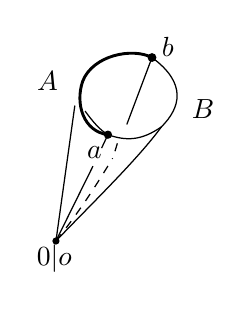
\begin{tikzpicture}[x=1cm,y=1cm,line width=.45pt]
\coordinate (o) at (0,0);
\coordinate (a) at (.66,1.35);
\coordinate (b) at (1.22,2.33);
\draw[line width=1.05pt] (a)
  .. controls (.35,1.39) and (.24,1.74) .. (.34,2.03)
  .. controls (.47,2.36) and (.97,2.46) .. (b);
\draw (.37,1.65) .. controls (.48,1.50) and (.56,1.41) .. (a);
\draw (b)
  .. controls (1.67,2.00) and (1.58,1.69) .. (1.34,1.45)
  .. controls (1.08,1.27) and (.89,1.27) .. (a);
\draw (o) -- (.24,1.72);
\draw (o) .. controls (.48,.50) and (1.04,1.04) .. (1.34,1.45);
\draw (b) -- (.90,1.48);
\draw[dashed] (o) .. controls (.36,.45) and (.59,.84) .. (.72,1.05);
\draw (.75,1.14) -- (.78,1.24);
\draw (o) -- (.47,.95);
\draw (a) -- (.58,1.18);
\fill (a) circle (1.5pt);
\fill (b) circle (1.6pt);
\fill (o) circle (1.3pt);
\node[left] at (.15,2.03) {$A$};
\node[right] at (1.60,1.67) {$B$};
\node at (.49,1.12) {$a$};
\node at (1.42,2.47) {$b$};
\node at (-.02,-.22) {$\unsure{0|o}$};
\end{tikzpicture}}}

For every $x\in X$, let us consider \inserted{the set $I_x\subset I$} of $i\in I$ such
that $X_i\ni x$ --- there are a finite number of them, \deleted{and}
(by (1' \unsure{a|0})), and the set of these $I$ is downward
filtering by (21 d), so there is
a least $i\in I_x$ \deleted{such that}, say $i(x)$
\[
(25)\qquad i(x)=\text{least of the }i\in I\text{ such that }x\in X_i.
\]
Let, on the other hand, for every $i\in I$
\margin{53}
